
\chapter{用户兴趣探索}
\label{chap:interestExplore}
电子商务产品的设计往往是数据驱动的,即许多产品方面的决策都是把用户行为量化后得出的。但就商品而言,那些热门主题往往只代表了用户一小部分的个性化需求,只有通过对用户行为的充分分析,才能更好的挖掘出用户的兴趣,最终提升商品的销售量。现有的推荐算法注重用户或资源间的相似性的同时却忽略了用户兴趣的动态变化,从而导致系统在时间维度上有偏离用户需求的趋势。

为了更好的探索用户兴趣,手机主题推荐系统充分利用了用户画像和商品特征表。用户画像包括基本信息和兴趣特征向量,商品特征向量表包括分类、标签、适用人群等,给定某用户行为,用户兴趣探索过程分为如下几个步骤:首先,利用用户历史行为(评论,停留时长,评分,点赞,购买等)建模量化用户满意度,然后,利用用户兴趣特征向量与商品特征向量得出相关分数,如果商品与用户的相关分数很低,但有很高的用户满意度,说明是一次成功的用户兴趣探索,更新用户画像。如果是热门商品,大量的用户都会点击,但商品与用户不是很相关,则认为其探索效果是有限的,反之如果是小众商品,考虑到长尾效应,则可以认为其是更成功的兴趣探索。这里涉及到的关键概念包括用户满意度的量化、小众标签的定向挖掘、用户兴趣的动态化。

本章内容首先介绍海量用户行为数据的存储方式。用户行为数据拥有区别于传统数据库数据的特点有,用户行为数据量巨大,常面临TB甚至PB级的数据;含有较多的噪音;多维聚合式查询。针对这些特征,用户行为数据采用Hbase数据集群存储和hadoop集群计算。然后,介绍用户兴趣探索的算法模型;然后,介绍如何通过用户行为的分析量化用户满意度。最后,介绍小众兴趣标签的挖掘。

\section{用户行为数据的存储}
手机主题用户行为数据的特点包括:用户基数庞大。手机主题注册用户达千万级,活跃用户达百万级;用户规模增长快。月新注册用户达10万数量级。每个用户的行为数量较小。即使是活跃用户,每天最多也只能产生上百条行为记录,每年不超过十万条;用户行为的计算较为复杂。计算用户的两次登录间隔天数、反复购买的商品、累积在线时间,这些都是针对用户行为的计算,通常具有一定的复杂性;用户行为数据格式不规整,字段丢失率较高。根据用户行为数据的这些特点,我们采用基于Hadop分布式的架构。
\begin{itemize}
\item 高可靠性。Hadoop按位存储和处理数据的能力使其具有高可靠性。
\item 高扩展性。Hadoop是在可用的计算机集簇间分配数据并完成计算任务的,这些集簇可以根据用户增长规模方便地扩展到数以千计的节点中。
\item 高容错性。Hadoop能够自动保存数据的多个副本,并且能够自动将失败的任务重新分配。
\item 高效性。Hadoop能够在节点之间动态地移动数据,并保证各个节点的动态平衡,因此处理速度非常快。
\item 低成本。hadoop是开源的,项目的软件成本因此会大大降低。
\end{itemize}

  \subsection{HDFS的体系架构}
  HDFS采用主从(Master/Slave)结构模型,一个HDFS集群是由一个NameNode和若干个DataNode组成的(在最新的Hadoop2.2版本已经实现多个NameNode的配置)。NameNode作为主服务器,管理文件系统命名空间和客户端对文件的访问操作。DataNode管理存储的数据。HDFS支持文件形式的数据。从内部来看,文件被分成若干个数据块,这若干个数据块存放在一组DataNode上。NameNode执行文件系统的命名空间,如打开、关闭、重命名文件或目录等,也负责数据块到具体DataNode的映射。DataNode负责处理文件系统客户端的文件读写,并在NameNode的统一调度下进行数据库的创建、删除和复制工作。NameNode是所有HDFS元数据的管理者,用户数据永远不会经过NameNode,HDFS体系结构图如\autoref{pic:hl_hadoop}所示。
  \begin{figure}
  \centering
    \framebox{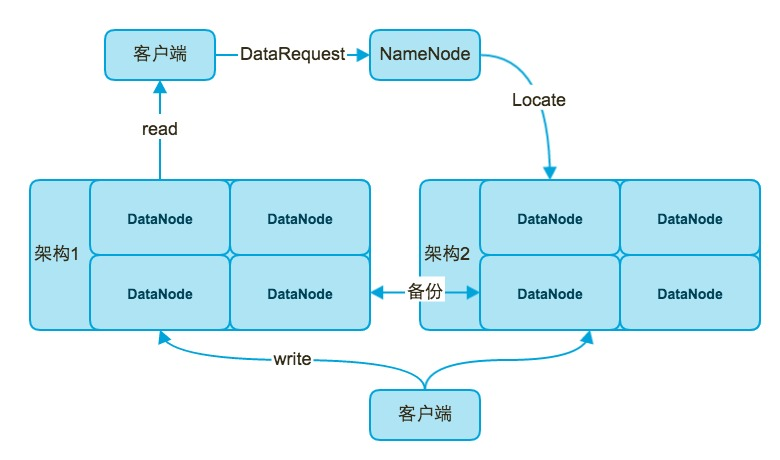
\includegraphics[scale=0.4]{figures/hl_hadoop}}
    \figcaption{HDFS体系结构}
    \label{pic:hl_hadoop}
  \end{figure}

  \subsection{Hive数据管理}
  HDFS为海量的数据提供了存储,则Hive支撑了海量的数据统计。Hive是建立在Hadoop上的数据仓库基础架构。它提供了一系列的工具,用来进行数据提取、转换、加载,是一种可以存储、查询和分析存储在Hadoop中的大规模数据机制。可以把Hadoop下结构化数据文件映射为一张成Hive中的表,并提供类sql查询功能,除了不支持更新、索引和事务,sql其它功能都支持。可以将sql语句转换为MapReduce任务进行运行,作为sql到MapReduce的映射器。提供shell、JDBC/ODBC、Thrift等接口。优点是成本低可以通过类sql语句快速实现简单的MapReduce统计。

本小节主要介绍了Hadoop分布式计算平台最核心的分布式文件系统HDFS以及数据仓库工具Hive。从体系架构到数据定义到数据存储再到数据处理,Hadoop分布式存储、计算平台为海量用户行为的分析和用户兴趣探索提供了可能。接下来的章节先介绍用户行为数据的分析,包括数据预处理和异常数据监测,然后介绍用户兴趣探索模块,包括算法模型、用户满意度量化、小众兴趣标签的挖掘。

\section{用户行为数据的的预处理}
数据预处理是数据挖掘过程中一个重要步骤,当原始数据存在不一致、重复、含噪声、维度高等问题时,更需要进行数据的预处理,以提高数据挖掘对象的质量,最终达到提高数据挖掘所获模式知识质量的目的。
  \subsection{背景}
  随着手机主题市场交易规模的逐步增大,积累下来的业务数据和用户行为数据越来越多,这些用户数据往往是电子商务平台最宝贵的财富。目前在手机主题推荐系统中大量地应用到了机器学习和数据挖掘技术,例如个性化推荐、搜索排序、用户画像建模等等,为企业创造了巨大的价值。本节主要介绍在用户兴趣探索实践中的数据预处理与特征挖掘方法。

  \subsection{特征提取}
  用户兴趣探索的任务包括:探索用户的兴趣广度、兴趣深度、兴趣变动趋势。依据这些信息,推荐系统就能知道在面对某一个用户时要推荐哪几类型商品,每类商品所占的比例,未来几天推荐内容会有哪些变化。在确定了目标之后,接下来需要确定使用哪些数据来达到目标。提取哪些特征数据可能与用户是否点击购买相关,一方面可以借鉴一些业务经验,另一方面可以采用一些特征选择、特征分析等方法。从业务经验来判断,可能影响用户是否点击下单的因素有:
  \begin{itemize}
  \item 用户历史行为。对于老用户,之前可能有过点击、购买等行为。
  \item 用户实时兴趣。
  \item 用户满意度。上面的特征都是比较好衡量的,用户满意度可能是更复杂的一个特征,具体体现在用户评分、评价、购买后使用频率、时长等。
  \item 是否热门,商品评价人数,购买数等。
  \end{itemize}
  在确定好要使用哪些数据之后,还需要对使用数据的可用性进行评估,包括数据的获取难度,数据的规模,数据的准确率,数据的覆盖率等。
  \begin{itemize}
  \item 用户历史行为。只有老用户才会有行为,新用户是没有的。
  \item 数据获取难度。获取用户id不难,但是获取用户年龄和性别较困难,因为用户注册或者购买时,这些并不是必填项,即使填了也不完全准确。如果一些特征需要通过其他预测模型交叉验证的话,就存在着模型精度的问题。
  \item 数据覆盖率。数据覆盖率也是一个重要的考量因素,例如地理位置特征,并不是所有用户的距离我们都能获取到,PC端的就没有地理位置,还有很多用户禁止使用它们的定位功能。
  \item 用户实时行为。如果用户刚打开app,还没有任何行为,同样面临着一个冷启动的问题。
  \item 数据的准确率。有时候用户购买一款主题,不一定是其真心喜欢,可能是因为遇到限时半价、购买返现等活动。
  \end{itemize}

  \subsection{特征获取方式}
  特征提取方式分为在线提取和离线提取。离线特征获取方案。离线可以使用海量的数据,借助于分布式文件存储平台,例如HDFS等,使用Spark等工具来计算海量的数据等。在线特征比较注重获取数据的延时,由于是在线服务,需要在非常短的时间内获取到相应的数据,对查找性能要求非常高,因此推荐系统输入流使用了Kafka,Kafka是一种分布式的,基于发布/订阅的消息系统。

  \subsection{用户行为数据预处理}
  原始服务器日志数据脏数据的形成原因包括:缩写词不统一,数据输入错误,不同的惯用语,重复记录,丢失值,不同的计量单位,过时的编码等。相应的,数据预处理内容包括数据清理、数据集成、数据变换、数据归约、数据离散化。

  1)数据清理包括格式标准化、异常数据清除、错误纠正、重复数据的清除。对于手机主题用户数据来讲,引起空缺值的原因主要是用户设备异常造成的,有些时候是因为与其他已有数据不一致而被删除或数据的改变没有进行日志记载。根据数据空缺情况的不同有不同的处理方式:
  \begin{itemize}
  \item 忽略元组。当一个记录中有多个属性值空缺、特别是关键信息丢失时,已不能反映真实情况,它的效果非常差。
  \item 去掉属性。缺失严重时,已无挖掘意义。
  \item 人工填写空缺值。但是工作量大且可行性低。
  \item 默认值。比如使用unknown或-∞。
  \item 使用属性的平均值填充空缺值。
  \item 预测最可能的值填充空缺值。使用贝叶斯公式或判定树这样的基于推断的方法。
  \end{itemize}

  2)数据集成就是将多个数据源中的数据整合到一个一致的存储中,需要注意以下几个情况:
  \begin{itemize}
  \item 模式集成。整合不同数据源中的元数据时的实体识别问题,比如匹配俩个表中的用户ID,A.custId=B.customerNo。
  \item 检测/解决数值冲突。对现实世界中的同一实体,来自不同数据源的属性值可能有所不同,如同表示停留时长,A表单位是秒,B表单位为毫秒。
  \item 多表之间的数据冗余。同一属性在不同的数据库中会有不同的字段名,有些时候冗余可以被相关分析检测出来,计算公式如所示,其中$\overline{A}$和$\overline{B}$表示为字段A和B的平均值,$\sigma_A和\sigma_B$表示其的标准差。仔细将多个数据源中的数据集成起来,能够减少或避免结果数据中的冗余与不一致性,从而可以提高挖掘的速度和质量。
  \begin{equation}
    r_{A,B} = \frac{\sum (A-\overline{A})(B-\overline{B})}{(n-1)\sigma_A\sigma_B}
    \label{F-Measure}
  \end{equation}
  \end{itemize}

  3)数据变换包括数据的平滑变换、数据聚集和数据规范化。所谓规范化是指将数据按比例缩放,使之落入一个小的特定区间,推荐系统采用了最小-最大规范化。如\autoref{equ:minMax}所示,原始数值范围为[min,max],通过公式映射到新区间[newMin,newMax],$v'$表示属性v的公式映射。

\section{用户兴趣探索的算法模型}
用户兴趣探索就是不断学习用户所感兴趣的内容反馈给个性化推荐模型去加强推送相关内容,本节首先介绍用户兴趣模型的基本概念,然后介绍算法模型的组成结构:用户异常兴趣探测,用户小众兴趣标签的挖掘和用户满意度量化,用户兴趣衰减算法。

  \subsection{基本概念概述}
  实体域。当我们想基于用户行为分析来建立用户兴趣模型时,我们必须把用户行为和兴趣主题限定在一个实体域上。个性化推荐落实在具体的推荐中都是在某个实体域的推荐。对于手机主题应用市场来说,实体域包括所有的主题,背景图片,铃声,闹铃等。

  用户行为。浏览,点击,下载,试用,购买,评论等都可是用户行为。本文所指的用户行为都是指用户在某实体域上的行为。比如用户在手机铃声产生的行为。
  
  用户兴趣。用户的兴趣维度,同样是限定在某实体域的兴趣,通常以标签+权重的形式来表示。比如,对于手机主题,用户兴趣向量可以是「动漫,0.6」,「体育,0.1」,「情感,0.7」等分类标签。值得一提的是,用户兴趣只是从用户行为中抽象出来的兴趣维度,并无统一标准。而兴趣维度的粒度也不固定,如「体育」,「电影」等一级分类,而体育下有「篮球」,「足球」等二级分类,篮球下有「NBA」,「CBA」,「火箭队」等三级分类。我们选取什么粒度的兴趣空间取决于具体业务模型。

  兴趣空间。在同一层次上兴趣维度的集合,比如手机主题中,可以用「热门」,「游戏」,「限时特价」,「科技」来构成一个程序员兴趣标签空间,也可以用「二次元」,「萝莉」,「魔幻」,「纯真」,「召唤兽」·····「法术」等构成一个动漫兴趣标签空间。

  \subsection{用户异常兴趣探测算法}
  本文所指的用户异常兴趣是指用户对小众标签主题表现出足够多的满意度。比如用户小磊每次都会浏览动漫、美少女主题,但是有一天却购买了一款汽车手机主题,那么程序可以检测到这种异常情况,然后将汽车标签更新到用户画像中,并作为个性化推荐的依据。事实上用户兴趣迭代过程可以在很短的时间内完成,基于 hive + MapReduce 平台的时长维度为天,而基于 kafka + spark 平台可以将时长维度降到小时级别。用户异常兴趣检测算法要从用户的行为和偏好中发现新的兴趣标签,并基于此给予推荐,工作内容包括收集用户的最新的行为数据是并分析得出异常标签,如\autoref{algo:newTagsExpore}所示
  \begin{algorithm}
  %% \SetLine
  \KwIn{用户画像数据 userProfile ,用户显示、隐式行为数据 logUsers}
  \KwOut{用户异常兴趣标签 newUsersTags}
  init newUsersTags;\\
  \For{$(user_i in logUsers)$}{
    \For{$(tag_j in user_i)$}{
      \If{$(tag_j.weight==0)$}{
        //若标签权重已经为 0,该用户兴趣标签将被删除\\
        remove $tag_j$;
      }
      \Else {
        //成功探测到新用户兴趣标签\\
        temp.get($user_i$).set($tag_j$);
      }
    } 
  }
  \Return temp;
  \caption{用户异常兴趣探测}
  \label{algo:newTagsExpore}
  \end{algorithm}

  \subsection{长尾标签抽取算法}
  标签集中度(tagFocus)是指,如果某个标签在一类主题中出现的频率高,其他主题类型很少出现,则认为此兴趣标签具有很好的类别区分能力。这是因为包含兴趣标签t的主题越少,也就是n越小,则说明标签t具有很好的兴趣区分,则其探索权重越大。如果某一类主题包C中包含兴趣标签t的个数为tagInThemeNum,而其它类包含t的总数为tagInOtherNum,则所有包含t的主题数n=tagInThemeNum+tagInOtherNum,当m大的时候,n也大,标签权重值会小,就说明该标签t类别区分能力不强。实际上,如果一个标签在一个类的主题中频繁出现,则说明该标签能够很好代表这类主题的特征,这样的标签应该给它们赋予较高的权重,并选来作为该类主题的特征向量以区别于其它类主题。热度(tagPopular)指的是某一个给定标签在用户画像中出现的频率。例如在300万用户总数中,十分之一的用户标签中有"火影"标签,那么其热度为0.1,除此之外有些标签如"精品","气质"等标签占了总词频的80\%以上,而它对区分主题类型几乎没有用。我们称这种词叫“应删标签”。即应删除词的权重应该是零,也就是说在度量相关性是不应考虑它们的频率。标签集中度公式如\autoref{equ:focus}所示,我们很容易发现,如果一个标签只在很少的主题包中出现,我们通过它就容易锁定搜索目标,它的权重也就应该大。反之如果一个词在大量主题包中出现,我们看到它仍然不很清楚要找什么内容,因此它应该小。热度公式如\autoref{equ:hot}所示。长尾标签抽取算法如\autoref{algo:longTailTags}所示。
    \begin{equation}
      tagFocus=log\frac{|tagInThemeNum|}{|tagInThemeNum+tagInOtherNum|}
      \label{equ:focus}
    \end{equation}

    \begin{equation}
      tagPopular=log\frac{|peopleLikeTagNum|}{|allPeople|}
      \label{equ:hot}
    \end{equation}

  \begin{algorithm}
  %% \SetLine
  \KwIn{用户画像数据 userProfile ,用户显示、隐式行为数据 logUsers}
  \KwOut{长尾兴趣标签 longTailTags}
  init longTailTags;\\
  \For{$(user_i in logUsers)$}{
    \For{$(tag_j in user_i)$}{
      $weight_{ij}$=$tag_j$.tagFocus/$tag_j$.tagPopular;\\
      \If{$(weight_{ij}<=threshold)$}{
        //若标签权重小于阈值,该用户兴趣标签将被删除\\
        remove $tag_j$;
      }
      \Else {
        //成功探测到新用户兴趣标签\\
        longTailTags.get($user_i$).set($tag_j$);
      }
    } 
  }
  \Return longTailTags;
  \caption{长尾兴趣探测}
  \label{algo:longTailTags}
  \end{algorithm}

  \subsection{用户满意度量化算法}
  要从用户的行为和偏好中量化用户满意度,并基于此实现兴趣标签探索,如何收集用户的偏好行为成为用户兴趣探索效果最基础的决定因素。用户有很多方式向系统提供自己的偏好信息,而且不同的应用也可能大不相同。
    \begin{table}[htp]
    \centering
    \tabcaption{用户行为和其权重}
    \label{tab:userAction}
    \begin{tabular}{ |c|c|p{4cm}|p{5cm}|c|} \hline
     用户行为 & 类型 & 特征 & 作用 & 权重\\ \hline
     评分 & 显式 & 整数量化的偏好,可能的取值是 [0, 5] & 通过用户对物品的评分,可以精确的得到用户的满意度,但是噪声比较大,比如遇到好评返现活动 & 1\\ \hline
     分享 & 显式 & 布尔量化的偏好,取值是 0 或 1 & 通过用户对物品的投票,可以精确的得到用户的喜好度,同时可以推理得到被转发人的兴趣取向(不太精确)& 2\\ \hline
     评论 & 显式 & 一段文字,需要进行文本分析,得到偏好 & 通过分析用户的评论,可以得到用户的情感:喜欢还是讨厌 & 1\\ \hline
     赞/踩 & 显示 & 布尔量化的偏好,取值是 0 或 1 & 带有很强的个人喜好度 & 3 \\ \hline
     购买、试用 & 显式 & 布尔量化的偏好,取值是 0 或 1 & 用户的购买是很明确的说明这个项目它感兴趣。& 3 \\ \hline
     点击流 & 隐式 & 包括滑屏频率,滑屏次数,屏停留时长,用户对物品感兴趣,需要进行分析,得到偏好 & 用户的点击一定程度上反映了用户的注意力,所以它也可以从一定程度上反映用户的喜好。& 1 \\ \hline
     停留时长 & 隐式 & 一组时间信息,噪音大,需 要进行去噪,分析,得到偏 好 & 用户的页面停留时间一定程度上反映了用户的注意力和喜好,但噪音偏大,不好利用。比如说用户在浏览一个主题的时候,丢下手机和同学出去踢球去了,页面提留时长可能会很长 & 1 \\ \hline
    \end{tabular}
    \end{table}
  \autoref{tab:userAction}列举的用户行为都是比较通用的,实际使用中提取的用户行为有数十种,根据不同行为反映用户喜好的程度将它们进行加权,得到用户对于物品的总体喜好。显式的用户反馈比隐式的权值大,但比较稀疏,毕竟进行显示反馈的用户是少数;而隐式用户行为数据是用户在使用应用过程中产生的,它可能存在大量的噪音和用户的误操作,可以通过经典的数据挖掘算法过滤掉行为数据中的噪音,这样可以使分析更加精确。然后是归一化操作,因为不同行为的数据取值可能相差很大,比如,用户的浏览数据必然比购买数据大的多,如何将各个行为的数据统一在一个相同的取值范围中,从而使得加权求和得到的总体喜好更加精确,就需要我们进行归一化处理使得数据取值在 [0,1] 范围中。算法如\autoref{algo:longTailTags}所示。

  \begin{algorithm}
  %% \SetLine
  \KwIn{用户显示、隐式行为数据 logUsers}
  \KwOut{用户行为权重 userActionWeight}
  init userActionWeight;\\
  \For{$(user_i in logUsers)$}{
    \For{$(action_j in user_i)$}{
      //获取用户此次行为的偏好权重并做归一化\\
      $weight_{ij}$=getWeigth($action_j$);
      \If{$(user_i exsit in userActionWeight)$}{
        //对用户行为做加权处理。\\
        double remaind=userActionWeight.get($user_i$);
        userActionWeight.get($user_i$).set(remaind+$action_j*weight_j$);
      }\Else{
        userActionWeight.get($user_i$).set($action_j*weight_j$);
      }
    } 
  }
  \Return userActionWeight;
  \caption{用户满意度量化算法}
  \label{algo:userActionWeight}
  \end{algorithm}

  \subsection{标签权重的线性衰减}
  标签权重的线性衰减算法结合了手机主题用户兴趣偏好变化频繁的特点,根据时间因素权重自动进行衰减,并准确反映用户兴趣的变化趋势。该模型是指用户对资源项目的评分仅代表评价当时的兴趣度,随着时间的推移,用户对该资源项目的评分将规律性地自动衰减,当项目评分衰减到 0 时,该资源项目将被兴趣模型所淘汰。评分衰减可以按照线性规律进行,如\autoref{pic:hl_lineReg}所示。算法描述如\autoref{algo:init_userProfile}所示。
  \begin{algorithm}
  %% \SetLine
  \KwIn{用户画像模型中所有用户兴趣哈希表 users{}}
  \KwOut{更新后的所有用户兴趣哈希表 users{}}
  \For{$(user_i in users)$}
  {
    //考虑到断电或意外关机等原因导致系统中断运行的特殊情况,算法加入了临时变量temp\\
    temp.add($user_i$.profile{});
  }
  \For{$(user_i in logUsers)$}
  {
    \For{$(tag_j in user_i)$}{
      \If{$(tag_j==0)$}{
        //若标签权重已经为 0,该用户兴趣标签将被删除\\
        remove $tag_j$;
      }\ElseIf {$(tag_j$ exsit in temp$(user_i)$}{
        //若存在新的评分值,则更新为新标签权重
        temp.get($user_i$).set($tag_j$);
      }\Else{
        //否则的话,将偏好值减少 0.5,进行衰减\\
        temp.get($user_i$).set($tag_j$-0.5);
      }
    }
  }
  \Return temp;
  \caption{用户画像线性衰减}
  \label{algo:init_userProfile}
  \end{algorithm}

  \begin{figure}
  \centering
    \framebox{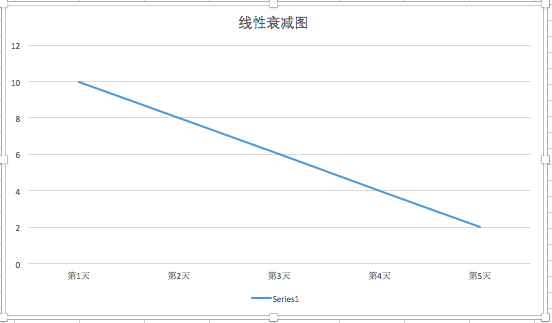
\includegraphics[scale=0.5]{figures/hl_lineReg}}
    \figcaption{线性衰减模型}
    \label{pic:hl_lineReg}
  \end{figure}

\section{用户兴趣探索评估方法}

  \subsection{线下测试}
  在太平洋东部加拉帕戈斯(Galapagos)的一个小岛上有一种名叫达尔文雀的鸟,一部分生活在岛的西部,另一部分生活在岛的东部,由于生活环境的细微不同它们进化出了不同的喙,如\autoref{pic:hl_abbird}所示,这被认为是自然选择学说上的一个重要例证。同样一种鸟,究竟哪一种喙更适合生存呢?自然界给出了她的解决方案,让鸟儿自己变异(设计多个方案),然后优胜劣汰。具体到达尔文雀这个例子上,不同的环境中喙也有不同的解决方案。
  \begin{figure}
  \centering
    \framebox{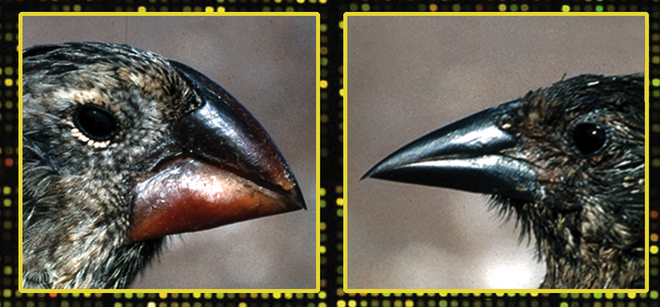
\includegraphics[scale=0.45]{figures/hl_abbird}}
    \figcaption{达尔文雀}
    \label{pic:hl_abbird}
  \end{figure}
  上面的例子包含了A/B测试最核心的思想:多个方案并行测试;每个方案只有一个变量(比如鸟喙)不同;以某种规则优胜劣汰。评判用户画像模型的效率高低,主要是看该模型带来的点击率、转换率等指标数据,其他统计量见\autoref{tab:abtest}所示。理论上评测推荐系统的指标有用户满意度、预测准确度、覆盖率、多样性、新颖度、惊喜度、信任度、实时性、健壮性等。然而商业开发中,评测推荐结果只看重一个指标:点击转化率。能够提升商业价值,给业务带来更多利益的推荐系统,就是好的推荐系统。
  \begin{table}[htp]
  \centering
  \tabcaption{A/B测试主要评估指标}
  \label{tab:abtest}
  \begin{tabular}{ |c|p{10cm}| } \hline
   指标 & 描述 \\ \hline
   访客数 & 访客数就是指一天之内到底有多少不同的用户访问了你的网站。访客数要比IP数更能真实准确地反映用户数量。\\ \hline
   浏览量 & 即Page View,浏览量和访问次数是呼应的。用户访问网站时每打开一个页面,就记为1个PV。同一个页面被访问多次,浏览量也会累积。 \\ \hline
   点击转化率 & 点击转化率计算公式:点击转化率 = 成交笔数/浏览量 *100\%,成交笔数影响着成交金额,所以点击转化率成为了衡量推荐系统效果的重要数据之一。\\ \hline
   停留时长 & 停留时长是用户访问网站的平均停留时间,是衡量网站用户体验的一个重要指标。如果用户不喜欢主题包的内容,可能稍微看一眼就关闭页面了,那么停留时长就很短;如果用户对页面的内容很感兴趣,停留时长就很长。\\ \hline
   跳出率 & 跳出率是指访客来到网站后,只访问了一个页面就离开网站的访问次数占总访问次数的百分比,跳出率越低说明流量质量越好,用户对网站的内容越感兴趣。 \\ \hline
   其他指标 & 各种辅助性指标如点击量/用户,购买量/用户,下载量/用户等。\\ \hline
  \end{tabular}
  \end{table}

  A/B测试对用户画像建模的作用有三个:特征提取,一些标签对用户的兴趣有强相关作用,如性别标签,有些标签是弱相关作用,如用户职业标签,A/B测试需要筛选出强相关标签,过滤掉弱相关标签;权重量化,根据A/B测试实验显示,发现用户画像中的最近点击标签、最近关注标签所占权重比想象中的要大;标签组合,有些标签是冗余的,只需从中选一即可。A/B测试具体实现步骤如下:

  \begin{itemize}
  \item 方案设计。实验之前需得到一个基准版本,然后把又争议的标签按照优先度列举出来决定是否实验。真正的A/B测试只应一次改动一个地方,这意味着标签选择、权重量化、标签组合要分开来测试。
  \item 确定数据评估方案。根据实验内容不同评估它们好坏的标准也不同,如果是标签选择那么衡量的主要指标是点击量,如果是权重量化那么衡量的主要指标是点击转换率。
  \item 流量分配。为了试实验所得数据具备统计意义,能准确反映用户的真实行为,需要对流量设置一个下限。除此之外,为了使各个方案具有可比性, A、B俩个方案的流量必须是相等的。
  \item 测试周期。根据所需测试的项目的不同测试周期也有所不同,如添加一个地理标签需要的测试周期以天为单位,如果涉及到多个标签的权重变动则需要测试周期以周为单位。
  \item 评估结果。适者胜出,其代表的数据作为下一轮回A/B测试的基准版本。
  \item 建立通用的数据评估题型。在经过各种类型A/B测试实验后,已经积累很多的评估指标,有必要把这些指标抽象出来形成一个通用的数据评估模型,减少以后实验的重复设计评估指标的时间。
  \end{itemize}

\section{总结}
这一章主要研究了标签动态变化的对推荐系统的影响,实际中用户同时会受到社会因素和个人因素的影响,但这两种因素在会产生不同强度的影响。在快速变化的系统中,用户行为更加会受到社会因素 的影响,而在变化相对较慢的系统中,用户行为则更加受到个人因素的影响。本章首先介绍了用户行为数据的存储方式以及基于此的用户行为数据的的预处理。然后介绍了用户兴趣探索的组成内容,包括用户异常兴趣探测、长尾标签抽取、用户满意度量化、标签权重的线性衰减。最后给出了用户兴趣探索评估方法,包括离线和在线俩种。下一章节主要介绍如何把用户画像和兴趣探索融入到推荐系统中,从而搭建出一个具有长尾性、实时性的推荐系统。